\documentclass{beamer}
%
% Choose how your presentation looks.
% For more themes, color themes and font themes, see:
% http://deic.uab.es/~iblanes/beamer_gallery/index_by_theme.html
%
\mode<presentation>
{
  \usetheme{Madrid}      % or try Darmstadt, Madrid, Warsaw, ...
  \usecolortheme{seahorse} % or try albatross, beaver, crane, ...
  \usefonttheme{serif}  % or try serif, structurebold, ...
  \setbeamertemplate{navigation symbols}{}
  \setbeamertemplate{caption}[numbered]
  \usepackage{amsmath}
  \usepackage{tcolorbox}
  \usepackage[export]{adjustbox}
  \tcbuselibrary{most}
  \usepackage{amsmath}  % conflicts with \oiint
  \usepackage{arydshln}
  \usepackage{tikz}
  \usetikzlibrary{plotmarks}
  \usepackage{pgfplots}
  \newcommand{\Ivec}[1]{\mbox{\boldmath $#1$}}
    \usepackage[normalem]{ulem}
    % \usepackage{tipa}
    \newcommand{\git}{\texttt{\textbf{git}}\xspace}
    \usepackage{listings}
} 


\definecolor{myblue}{RGB}{65,105,225} 
\definecolor{myorange}{RGB}{250,190,0}

\setbeamercolor{structure}{fg=white,bg=myorange}
\setbeamercolor*{palette primary}{fg=myblue,bg=myorange}
\setbeamercolor*{palette secondary}{fg=white,bg=myblue}
\setbeamercolor*{palette tertiary}{bg=myblue,fg=white}
\setbeamercolor*{palette quaternary}{fg=white,bg=myorange!50}

\setbeamercolor{frametitle}{fg=black!90!myblue}

\setbeamercolor{section in head/foot}{fg=white,bg=myblue}
\setbeamercolor{author in head/foot}{fg=black,bg=myorange}
\setbeamercolor{title in head/foot}{fg=white,bg=myblue}

\setbeamertemplate{navigation symbols}{}

\setbeamertemplate{itemize/enumerate body begin}{\large}
\setbeamertemplate{itemize/enumerate subbody begin}{\large}


\defbeamertemplate*{headline}{mytheme}
{%
  \begin{beamercolorbox}[ht=2.25ex,dp=3.75ex]{section in head/foot}
    \insertnavigation{\paperwidth}
  \end{beamercolorbox}%
}%

\defbeamertemplate*{footline}{mytheme}
{
  \leavevmode%
  \hbox{%
  \begin{beamercolorbox}[wd=.5\paperwidth,ht=2.25ex,dp=1ex,right]{author in head/foot}%
    \usebeamerfont{author in head/foot}\insertshortauthor\hspace*{2em}
  \end{beamercolorbox}%
  \begin{beamercolorbox}[wd=.5\paperwidth,ht=2.25ex,dp=1ex,left]{title in head/foot}%
    \usebeamerfont{title in head/foot}\hspace*{2em}\insertshortsubtitle\hspace*{2em}
    \insertframenumber{} / \inserttotalframenumber
  \end{beamercolorbox}}%
  \vskip0pt%
}

\usepackage[english]{babel}
\usepackage[utf8x]{inputenc}
\usepackage{xcolor}
\usepackage{listings}
\usepackage{pgf}  
\usepackage{textpos}
\usepackage{tabulary}
\usepackage{scrextend}
\usepackage{hyperref}
\usepackage{setspace}
\usepackage{rotating}
\lstset
{
    language=[LaTeX]TeX,
    breaklines=true,
    basicstyle=\tt\scriptsize,
    %commentstyle=\color{green}
    keywordstyle=\color{blue},
    %stringstyle=\color{black}
    identifierstyle=\color{magenta},
}
\newcommand{\bftt}[1]{\textbf{\texttt{#1}}}
%\newcommand{\comment}[1]{{\color[HTML]{008080}\textit{\textbf{\texttt{#1}}}}}
\newcommand{\cmd}[1]{{\color[HTML]{008000}\bftt{#1}}}
\newcommand{\bs}{\char`\\}
\newcommand{\cmdbs}[1]{\cmd{\bs#1}}
\newcommand{\lcb}{\char '173}
\newcommand{\rcb}{\char '175}
\newcommand{\cmdbegin}[1]{\cmdbs{begin\lcb}\bftt{#1}\cmd{\rcb}}
\newcommand{\cmdend}[1]{\cmdbs{end\lcb}\bftt{#1}\cmd{\rcb}}

\newcommand{\wllogo}{\textbf{Overleaf}}

\usepackage{hyperref}
\hypersetup{
    colorlinks=true,
    linkcolor=blue,
    filecolor=magenta,      
    urlcolor=cyan,
    pdftitle={Overleaf Example},
    pdfpagemode=FullScreen,
    }

\urlstyle{same}

% this is where the example source files are loaded from
% do not include a trailing slash
\newcommand{\fileuri}{https://raw.githubusercontent.com/GiancarloSucci/UniBo.IDSEPC.A2022/main/A2022.IDSEPCLaTeX/}

\newcommand{\perche}{perch\'{e}}
\newcommand{\affinche}{affinch\'{e}}
\newcommand{\se}{s\'{e}}
\newcommand{\a}{\`{a}}
\newcommand{\est}{\`{e}}

\usepackage{stackengine}
\def\Ruble{\stackengine{.67ex}{%
  \stackengine{.48ex}{\textsf{P}}{\rule{.8ex}{.12ex}\kern.6ex}{O}{r}{F}{F}{L}%
  }{\rule{.8ex}{.12ex}\kern.6ex}{O}{r}{F}{F}{L}\kern-.1ex}



%----------------------------------------------------------------------------------------
%	TITLE PAGE
%----------------------------------------------------------------------------------------
\title[L02]{Introduzione alla data science e al pensiero computazionale\\
Lezione 10: Correlazione} % The short title appears at the bottom of every slide, the full title is only on the title page

\author[{\tiny Giancarlo Succi }]{Giancarlo Succi\\\\ Dipartimento di Informatica -- Scienza e Ingegneria\\Universit\`{a} di Bologna\\
\bftt{g.succi@unibo.it}
} % Your name
\institute[unibo] % Your institution as it will appear on the bottom of every slide, may be shorthand to save space

\date{} % Date, can be changed to a custom date

\setbeamertemplate{navigation symbols}{}
\AtBeginSection[]
{
        \begin{frame}<beamer>{Outline}
                \tableofcontents[currentsection]
        \end{frame}
}

\begin{document}
\begin{frame}
\titlepage % Print the title page as the first slide

\end{frame}

\begin{frame}
{\centerline{Content}}

\begin{itemize}
\item Covariance
\item Correlation (aka Pearson product-moment correlation coefficient)
\item Relationship between Pearson correlation and linear regression
\end{itemize}
\end{frame}


\begin{frame}
{\centerline{Covariance}}

\begin{itemize}
\item To proceed further with our analysis we will use the concept of \textbf{covariance}, which we have already seen
\item It expresses the degree in which the variation of a random variable is connected to the variation of another random variable
\item It is defined as follows:
\begin{itemize}
\item Given two random variables $X$ and $Y$
$$Cov(X,Y) = E[ (X - E(X))(Y - E(Y))]$$
\end{itemize}
\end{itemize}

\end{frame}


\begin{frame}
{\centerline{Covariance -- graphically}}


\begin{center}
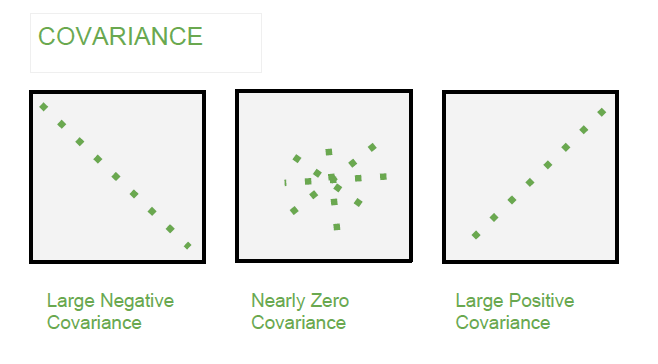
\includegraphics[width=10cm]{A2022.IDSEPC.Correlazione/Covar.png}
\end{center} 
\textit{\small
Source : \url{https://www.geeksforgeeks.org/mathematics-covariance-and-correlation}}
\end{frame}


\begin{frame}
{\centerline{About the covariance - 1}}

\begin{itemize}
\item We notice that:
\begin{itemize}
\item The covariance of a random variable with itself is the variance:
$$Cov(X,X) = Var(X)$$
\item There is a similar property as for the variance
$$Cov(X,Y) = E(XY) - E(X)E(Y)$$
since:
$$Cov(X,Y) = E[ (X - E(X))(Y - E(Y))] = $$
$$ = E(XY) - E(XE(Y)) - E(E(X)Y) + E(E(X)E(Y)) =$$
$$ = E(XY) - E(X)E(Y) - E(X)E(Y) + E(X)E(Y) = $$
$$ = E(XY) - E(X)E(Y)$$
QED.


\end{itemize}


\end{itemize}

\end{frame}


\begin{frame}
{\centerline{About the covariance - 2}} \label{P:Covariance2}

\begin{itemize}
\item The covariance is symmetric:
 $$Cov(X,Y) = Cov(Y,X)$$
\item The covariance is linear with respect to multiplications by constants:
 $$(\forall a, b \in \mathbb{R}) ~~ Cov(aX,bY) = abCov(X,Y)$$

\item If $e \sim N(0,\sigma)$, $Cov(X,e) = 0$ \\
$$Cov(X,e) =  E(Xe) - E(X)E(e)$$
Since  $X$ and $e$ are independent
$$ E(Xe) = E(X)E(e)$$
Moreover,  $e \sim N(0,\sigma)$
$$E(e) = 0$$
QED.
\end{itemize}


\end{frame}


\begin{frame}
{\centerline{Pearson Correlation Coefficient}} \label{P:Pearson}

\begin{itemize}
\item AKA Pearson product-moment correlation coefficient or just correlation coefficient
\item It expresses the linear correlation between two random variables
\item It is defined as follows:
\begin{itemize}
\item Given two random variables $X$ and $Y$
$$r_{X,Y} = \frac{Cov(X,Y)}{\sigma_X\sigma_Y}$$
\item Where:
$$\sigma_Z = \sqrt{Var(Z)}$$
\end{itemize}
\end{itemize}

\vspace*{0.5cm}

\textit{\small For the time being we intentionally ignore the difference between sample and population.}

\end{frame}

\begin{frame}
{\centerline{Pearson Correlation Coefficient -- graphically}}


\begin{center}
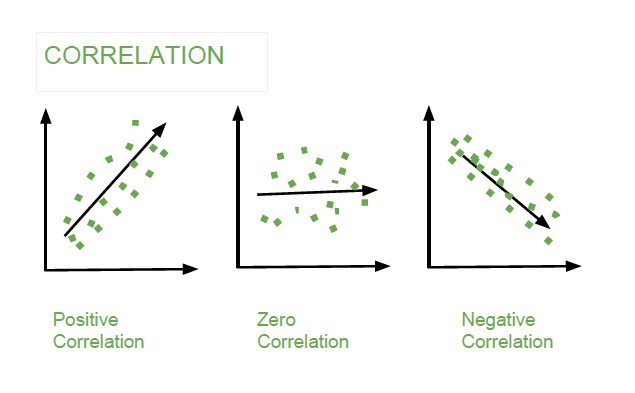
\includegraphics[width=10cm]{A2022.IDSEPC.Correlazione/Correl.png}
\end{center} 
\textit{\small
Source : \url{https://www.geeksforgeeks.org/mathematics-covariance-and-correlation}}
\end{frame}


\begin{frame}
{\centerline{About the Pearson Correlation Coefficient}}

\begin{itemize}
\item The Pearson correlation coefficient is also often expressed as:

$$ r_{X,Y} = \frac{\sum_{i=1}^{n}(x_i-\overline{x})(y_i-\overline{y})}{\sqrt{\sum_{i=1}^{n}(x_i-\overline{x})^2\sum_{i=1}^{n}(y_i-\overline{y})^2}} $$
\item It is symmetric: $r_{X,Y} = r_{Y,X}$
\item It is invariant with respect to multiplications by, and additions of constants: $(\forall a, b, c, d \in \mathbb{R} , b \neq 0, d \neq 0)~~ r_{X,Y} = r_{(a + bX),(c + dY)} $
\item It ranges from -1 to 1: $-1 \leq r_{X,Y} \leq 1$
$ r_{X,Y}=1$ means perfect linear relationship (all points lie on a monotonically increasing line) \\
$ r_{X,Y}=-1$ means perfect opposite linear relationship (all points lie on a monotonically decreasing line)\\
$ r_{X,Y}= 0$ means no linear relationship between $X$ and $Y$
\end{itemize}


\end{frame}

% ============= =========== % ============= ===========
\begin{frame}
{\centerline{Back to Linear Regression (1/2)}}
\begin{itemize}
\item We now focus our attention to the case of the case of the linear regression
\item Suppose we have two phenomena that we want to measure,  $X$ and $Y$
\item Let us assume 
\begin{itemize}
\item that there is a linear relationship between them
\item that I can express the data I collect as:
$$ \boldsymbol y = \boldsymbol \theta_0 + X  \boldsymbol \theta_1 + \boldsymbol \epsilon $$
\item where $\epsilon$ is a stationary gaussian process $N(0,\sigma^2)$
\end{itemize}
\item We know the solution that minimizes the square error
\end{itemize}
\end{frame}
% ============= =========== % ============= ===========

% ============= =========== % ============= ===========
\begin{frame}
{\centerline{Back to Linear Regression (2/2)}}
\begin{itemize}
\item From this solution we have extracted the coefficient of determination
$$R^2 = 1 - \frac{SS_{res}}{SS_{tot}}$$
\item Where: 
\begin{itemize}
\item $SS_{res} = \sum_i (y_i - \hat{y}_i)^2$ 
\item \textcolor{blue}{$SS_{res} $ is the distance between the reality and the 1-degree best approximation, that is, the OLS model}
\end{itemize}
\item and
\begin{itemize}
\item $SS_{tot} = \sum_i (y_i - \overline{y})^2$
\item  \textcolor{blue}{$SS_{tot}$ is the distance between the reality and the 0-degree best approximation, that is, the mean}
\end{itemize}

\item I want to know the relationship between $R^2$ and the correlation coefficient between $X$ and $Y$, $r_{X,Y}$
\end{itemize}
\end{frame}
% ============= =========== % ============= ===========

% ============= =========== % ============= ===========
\begin{frame}
{\centerline{Our goal -- understanding R and r}}
\begin{itemize}
\item We focus on 1D
\item We are now going to prove a fundamental point.
\item Under the assumption that the noise is gaussian and centered in 0, in a linear regression:
\end{itemize}
$$R^2 = r_{X,Y}^2$$
\end{frame}
% ============= =========== % ============= ===========


% ============= =========== % ============= ===========
\begin{frame}
{\centerline{$R^2 = r_{X,Y}^2$ (1/4)}}
\begin{itemize}
\item Since
$$ \hat{y} = \theta_0 + \theta_1 x$$
\item we have from above (see page \ref{P:Pearson}) that:
$$r_{X,Y} = r_{\hat{Y},Y}$$
\item We define now the explained sum of squares (ESS) 
\begin{itemize}
\item $ ESS = \sum_i (\hat{y}_i - \overline{y})^2$
\item \textcolor{blue}{$ ESS $ is the additional knowledge we get on the random variable using a polynomial of degree 1 vs. using a polynomial of degree 0}
\end{itemize}

\item We will now prove that \textbf{under our hypotheses}:
$$ESS + SS_{res} = SS_{tot} $$
\end{itemize}
\end{frame}
% ============= =========== % ============= ===========


% ============= =========== % ============= ===========
\begin{frame}
{\centerline{ [$R^2 = r_{X,Y}^2$] -- $ESS + SS_{res} = SS_{tot} $ (1/6)}}

\begin{itemize}
\item We start from:
$$(y_{i}-{\overline {y}})=(y_{i}-{\hat {y}}_{i})+({\hat {y}}_{i}-{\overline {y}})$$

\item which we square:
$$(y_{i}-{\overline {y}})^2=(y_{i}-{\hat {y}}_{i})^2 + 2(y_{i}-{\hat {y}}_{i})({\hat {y}}_{i}-{\overline {y}}) + ({\hat {y}}_{i}-{\overline {y}})^2$$

\item and then we sum:
$$\sum_i(y_{i}-{\overline {y}})^2=\sum_i(y_{i}-{\hat {y}}_{i})^2 + \sum_i2(y_{i}-{\hat {y}}_{i})({\hat {y}}_{i}-{\overline {y}}) + \sum_i({\hat {y}}_{i}-{\overline {y}})^2$$


\end{itemize}

\textit{\small
Source with modifications: \url{https://en.wikipedia.org/wiki/Explained_sum_of_squares}}
\end{frame}
% ============= =========== % ============= ===========

% ============= =========== % ============= ===========
\begin{frame}
{\centerline{ [$R^2 = r_{X,Y}^2$] -- $ESS + SS_{res} = SS_{tot} $ (2/6)}}

\begin{itemize}
\item Now we focus on:
$$\sum_i2(y_{i}-{\hat {y}}_{i})({\hat {y}}_{i}-{\overline {y}}) = 2\sum_i(y_{i}-{\hat {y}}_{i})({\hat {y}}_{i}-{\overline {y}}) $$
\item and we want to prove that it is 0, that is $\sum_i(y_{i}-{\hat {y}}_{i})({\hat {y}}_{i}-{\overline {y}}) = 0$;  considering:
$$y_i = \hat{y_i} + \epsilon_i$$
$$ E(y_i) = E(\hat{y_i} + \epsilon_i) = E(\hat{y_i}) + E(\epsilon_i) = E(\hat{y_i}) $$
because $\epsilon$ is a stationary gaussian process $N(0,\sigma^2)$

\end{itemize}

\textit{\small
Source with modifications: \url{https://en.wikipedia.org/wiki/Explained_sum_of_squares}}
\end{frame}
% ============= =========== % ============= ===========

% ============= =========== % ============= ===========
\begin{frame}
{\centerline{ [$R^2 = r_{X,Y}^2$] -- $ESS + SS_{res} = SS_{tot} $ (3/6)}}

\begin{itemize}
\item We can build a system:
\[
\systeme*{
\hat{y}_i = \theta_0 + \theta_1 x_i,
\overline{y} = \theta_0 + \theta_1 \overline{x}
}
\]
\item from which we deduce by subtraction:
$$\hat{y}_i - \overline{y} = \theta_1 (x_i - \overline{x})$$
\item remembering that:
$$ \theta_1  = \frac { Cov(x,y)} { Var(x) } = {\frac {\sum _{i=1}^{n}(x_{i}-{\overline {x}})(y_{i}-{\overline {y}})}{\sum _{i=1}^{n}(x_{i}-{\overline {x}})^{2}}}$$
\end{itemize}

\textit{\small
Source with modifications: \url{https://en.wikipedia.org/wiki/Explained_sum_of_squares}}
\end{frame}
% ============= =========== % ============= ===========


% ============= =========== % ============= ===========
\begin{frame}
{\centerline{ [$R^2 = r_{X,Y}^2$] -- $ESS + SS_{res} = SS_{tot} $ (4/6)}}

\begin{itemize}
\item So:
$$\sum_i(y_{i}-{\hat {y}}_{i})({\hat {y}}_{i}-{\overline {y}}) = \sum_i(y_{i}-{\hat {y}}_{i})(\theta_1 (x_i - \overline{x}))=$$
$$= \theta_1 \sum_i(y_{i}-{\hat {y}}_{i})(x_i - \overline{x})$$
\item Now, let's consider that:
$$(y_{i}-{\hat {y}}_{i})= y_{i}-{\hat {y}}_{i} + \overline {y} - \overline {y} = (y_{i}-{\overline {y}})-({\hat {y}}_{i}-{\overline {y}})= $$
$$ = (y_{i}-{\overline {y}})-{\theta_1}(x_{i}-{\overline {x}})$$
\item Substituting $(y_{i}-{\hat {y}}_{i})$ above we get:
$$ \theta_1 \sum_i(y_{i}-{\hat {y}}_{i})(x_i - \overline{x})=\theta_1 \sum_i[(y_{i}-{\overline {y}})-{\theta_1}(x_{i}-{\overline {x}}) ](x_i - \overline{x}) $$


\end{itemize}

\textit{\small
Source with modifications: \url{https://en.wikipedia.org/wiki/Explained_sum_of_squares}}
\end{frame}
% ============= =========== % ============= ===========

% ============= =========== % ============= ===========
\begin{frame}
{\centerline{ [$R^2 = r_{X,Y}^2$] -- $ESS + SS_{res} = SS_{tot} $ (5/6)}}

\begin{itemize}
\item We can conclude:
$$ \theta_1 \sum_i[(y_{i}-{\overline {y}})-{\theta_1}(x_{i}-{\overline {x}}) ](x_i - \overline{x}) = $$
$$ = \theta_1 [\sum_i (y_{i}-{\overline {y}}) (x_i - \overline{x}) -
\sum_i{\theta_1}(x_{i}-{\overline {x}}) (x_i - \overline{x})] = $$
$$ = \theta_1 [\sum_i (y_{i}-{\overline {y}}) (x_i - \overline{x}) -
\sum_i{{\frac {\sum _{j}(x_{j}-{\overline {x}})(y_{j}-{\overline {y}})}{\sum _{j}(x_{j}-{\overline {x}})^{2}}}
}(x_{i}-{\overline {x}})^2] = $$


\end{itemize}

\textit{\small
Source with modifications: \url{https://en.wikipedia.org/wiki/Explained_sum_of_squares}}
\end{frame}
% ============= =========== % ============= ===========

\begin{frame}
{\centerline{ [$R^2 = r_{X,Y}^2$] -- $ESS + SS_{res} = SS_{tot} $ (6/6)}}

\begin{itemize}
\item And simplifying what is in [ $\bullet$ ]:

$$ \sum_i (y_{i}-{\overline {y}}) (x_i - \overline{x}) -
\sum_i{{\frac {\sum _{j}(x_{j}-{\overline {x}})(y_{j}-{\overline {y}})}{\sum _{j}(x_{j}-{\overline {x}})^{2}}}
}(x_{i}-{\overline {x}})^2 = $$
$$=  \sum_i (y_{i}-{\overline {y}}) (x_i - \overline{x}) -
\sum _{j}(x_{j}-{\overline {x}})(y_{j}-{\overline {y}})\sum_i{{\frac {(x_{i}-{\overline {x}})^2}{\sum _{j}(x_{j}-{\overline {x}})^{2}}}
}= $$
$$=  \sum_i (x_i - \overline{x}) (y_{i}-{\overline {y}})  -
\sum _{j}(x_{j}-{\overline {x}})(y_{j}-{\overline {y}}){\frac {\sum_i{(x_{i}-{\overline {x}})^2}}{\sum _{j}(x_{j}-{\overline {x}})^{2}}} = $$
$$=  \sum_i (x_i - \overline{x}) (y_{i}-{\overline {y}})  -
\sum _{j}(x_{j}-{\overline {x}})(y_{j}-{\overline {y}}) = 0 $$


QED.


\end{itemize}

\textit{\small
Source with modifications: \url{https://en.wikipedia.org/wiki/Explained_sum_of_squares}}
\end{frame}
% ============= =========== % ============= ===========


% ============= =========== % ============= ===========
\begin{frame}
{\centerline{$R^2 = r_{X,Y}^2$ (2/4)}}
\begin{itemize}
\item Now we know that, under the assumption to deal with a Gaussian noise centered in 0 we have:
$$ESS + SS_{res} = SS_{tot} $$
\item Under this hypothesis we have:
$$R^2 = 1 - \frac{SS_{res}}{SS_{tot}} = \frac{SS_{tot}-SS_{res}}{SS_{tot}} = \frac{ESS}{SS_{tot}} $$
\end{itemize}
\end{frame}
% ============= =========== % ============= ===========

% ============= =========== % ============= ===========
\begin{frame}
{\centerline{$R^2 = r_{X,Y}^2$ (3/4)}}
\begin{itemize}
\item We now consider the square of $r_{X,Y} = r_{\hat{Y},Y}$
$$r_{\hat{Y},Y}^2= \left ( \frac{Cov(\hat{Y},Y)}{\sqrt{Var(Y)Var(\hat{Y})}} \right )^2 =  \frac{Cov(\hat{Y},Y)Cov(\hat{Y},Y)}{Var(Y)Var(\hat{Y})} = $$
$$ = \frac{Cov(\hat{Y},\hat{Y} + \epsilon)Cov(\hat{Y},\hat{Y} + \epsilon)}{Var(Y)Var(\hat{Y})} = $$
$$ 
= \frac{(Cov(\hat{Y},\hat{Y})+ Cov(\hat{Y},\epsilon))(Cov(\hat{Y},\hat{Y})+ Cov(\hat{Y},\epsilon))}{Var(Y)Var(\hat{Y})} = $$
$$ 
= \frac{Cov(\hat{Y},\hat{Y})Cov(\hat{Y},\hat{Y})}{Var(Y)Var(\hat{Y})} $$


\end{itemize}

\textit{\small
Source with modifications: \url{https://economictheoryblog.com/2014/11/05/proof/}}
\end{frame}
% ============= =========== % ============= ===========
% ============= =========== % ============= ===========
\begin{frame}
{\centerline{$R^2 = r_{X,Y}^2$ (4/4)}}
\begin{itemize}
\item But we know that $Cov(\hat{Y},\hat{Y}) = Var(\hat{Y})$, therefore we get that
$$r_{X,Y}^2 = \frac{Var(\hat{Y})Var(\hat{Y})}{Var(Y)Var(\hat{Y})} = \frac{Var(\hat{Y})}{Var(Y)}=$$
$$ = \frac{\frac{\sum_i{(\hat{y_i}-\overline{\hat{y}})^2}}{n}}{\frac{\sum_i(y_i-\overline{y})^2}{n}}
= \frac{{\sum_i{(\hat{y_i}-\overline{\hat{y}})^2}}}{\sum_i(y_i-\overline{y})^2} =  \frac{ESS}{SS_{tot}} $$
since we have already proven that $\overline{y} = \overline{\hat{y}}$
\end{itemize}
QED

\textit{\small
Source with modifications: \url{https://economictheoryblog.com/2014/11/05/proof/}}
\end{frame}
% ============= =========== % ============= ===========

% ============= =========== % ============= ===========
\begin{frame}
{\centerline{Comment on $R^2 = r_{X,Y}^2$ }}
\begin{itemize}
\item This is a major result\\
\item It is the center of our subsequent investigation, in the case of normality of error we can model, interconnect, and understand relationships in an easy way\\
\item The next question is on how the slope of the regression line ($\theta_1$) relates to the correlation coefficient $r_{X,Y}$

\end{itemize}

\end{frame}
% ============= =========== % ============= ===========

\begin{frame}
{\centerline{$ r_{X,Y} $ and $\theta_1$}}
\begin{itemize}
\item We know that:
$$ \theta_1  = \frac { Cov(X,Y)} { Var(X) } $$
\item And that:
$$r_{X,Y} = \frac{Cov(X,Y)}{\sigma_X\sigma_Y}$$
\item Therefore:
$$ \theta_1  Var(X) = r_{X,Y}  \sigma_X\sigma_Y $$
\item We can then conclude that:
$$ \theta_1  = \frac{\sigma_X\sigma_Y}{Var(X)} r_{X,Y}   $$
$$ r_{X,Y}   = \frac{Var(X)}{\sigma_X\sigma_Y} \theta_1  $$

\end{itemize}

\end{frame}
% ============= =========== % ============= ===========

% ============= =========== % ============= ===========

\begin{frame}
{\centerline{Comment on $ r_{X,Y} ~ \sim ~ \theta_1$}}
\begin{itemize}
\item $ r_{X,Y} $ and $\theta_1$ are therefore directly and monotonically proportional
\item It means that a positive relationships implies a positive slope and viceversa
\end{itemize}

\end{frame}
% ============= =========== % ============= ===========


% https://en.wikipedia.org/wiki/Explained_sum_of_squares


\begin{frame}
{\centerline{General remark}}

\begin{itemize}
\item Right now we work with samples of larger populations of data
\item We measure properties of samples, like mean, standard deviation, covariance, correlation coefficient
\item All these properties are also random variable and have a distribution
\item Our question is therefore, what kind of distribution is the one of the correlation coefficient
\item Knowing its distribution allows us to understand the relationships existing between the variables it connect
\end{itemize}


\end{frame}



\begin{frame}
{\centerline{Domande?}}
\vspace{1cm}
\begin{center}
    \LARGE{Fine della lezione dieci.}
\end{center}

\end{frame}


%----------------------------------------------------------------------------------------
\end{document}
